\documentclass[tikz]{standalone}

\usetikzlibrary{positioning,calc,matrix}
\usepackage{xcolor}

\tikzset{ 
table/.style={
  matrix of nodes,
  %row sep=-\pgflinewidth,
  row sep=2pt,
  column sep=-\pgflinewidth,
  nodes={rectangle,text width=5ex,align=center},
  text depth=0.75ex,
  text height=1.75ex,
  nodes in empty cells
  },
%texto/.style={font=\footnotesize\sffamily},
%title/.style={font=\small\sffamily}
}

\tikzset{XOR/.style={draw,circle,append after command={
        [shorten >=\pgflinewidth, shorten <=\pgflinewidth,]
        (\tikzlastnode.north) edge (\tikzlastnode.south)
        (\tikzlastnode.east) edge (\tikzlastnode.west)
        }
    }
}

\begin{document}
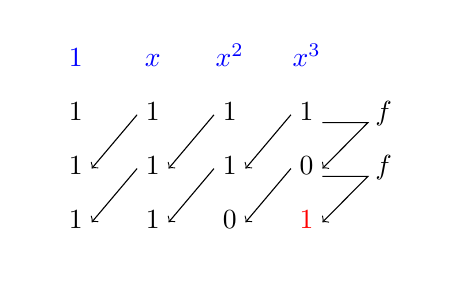
\begin{tikzpicture}
    \matrix [table] (p3)
    {
        {\color{blue}1} & {\color{blue}$x$} & {\color{blue}$x^2$} & {\color{blue}$x^3$} & \\
        1 & 1 & 1 & 1 & $f$ \\
        1 & 1 & 1 & 0 & $f$ \\
        1 & 1 & 0 & {\color{red}1} & \\
    };
    \foreach \i in {2, 3}
    {   
        \pgfmathtruncatemacro{\ii}{\i+1}
        \foreach \x in {2, 3, 4}
        {
            \pgfmathtruncatemacro\xx{\x-1}
            \draw [->] ($(p3-\i-\x.center)+(-.2cm,0)$) -- ($(p3-\ii-\xx.center)+(.2cm,0)$);
        }
        \draw [->] ($(p3-\i-4.center)+(.2cm,-.1cm)$) -- ($(p3-\i-5.center)+(-.2cm,-.1cm)$) -- ($(p3-\ii-4.center)+(.2cm, 0)$);
    }
    
\end{tikzpicture}

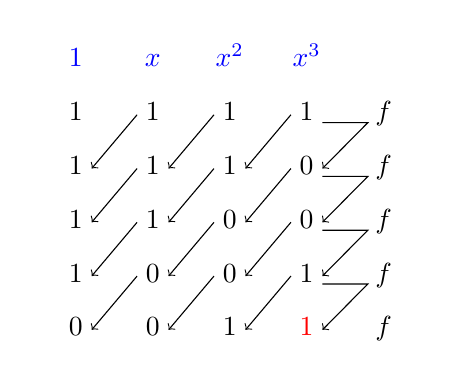
\begin{tikzpicture}
    \matrix [table] (p3)
    {
        {\color{blue}1} & {\color{blue}$x$} & {\color{blue}$x^2$} & {\color{blue}$x^3$} & \\
        1 & 1 & 1 & 1 & $f$ \\
        1 & 1 & 1 & 0 & $f$ \\
        1 & 1 & 0 & 0 & $f$ \\
        1 & 0 & 0 & 1 & $f$ \\
        0 & 0 & 1 & {\color{red}1} & $f$ \\
    };
    \foreach \i in {2, 3, 4, 5}
    {   
        \pgfmathtruncatemacro{\ii}{\i+1}
        \foreach \x in {2, 3, 4}
        {
            \pgfmathtruncatemacro\xx{\x-1}
            \draw [->] ($(p3-\i-\x.center)+(-.2cm,0)$) -- ($(p3-\ii-\xx.center)+(.2cm,0)$);
        }
        \draw [->] ($(p3-\i-4.center)+(.2cm,-.1cm)$) -- ($(p3-\i-5.center)+(-.2cm,-.1cm)$) -- ($(p3-\ii-4.center)+(.2cm, 0)$);
    }
    
\end{tikzpicture}

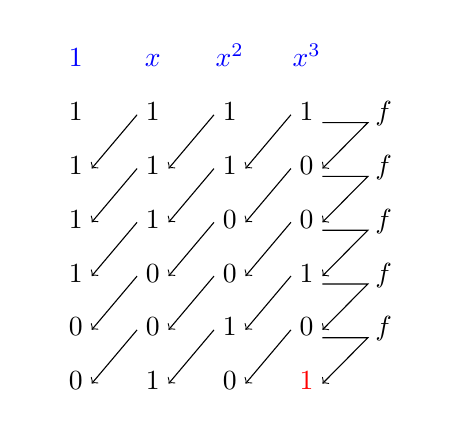
\begin{tikzpicture}
    \matrix [table] (p3)
    {
        {\color{blue}1} & {\color{blue}$x$} & {\color{blue}$x^2$} & {\color{blue}$x^3$} & \\
        1 & 1 & 1 & 1 & $f$ \\
        1 & 1 & 1 & 0 & $f$ \\
        1 & 1 & 0 & 0 & $f$ \\
        1 & 0 & 0 & 1 & $f$ \\
        0 & 0 & 1 & 0 & $f$ \\
        0 & 1 & 0 & {\color{red}1} & \\
    };
    \foreach \i in {2, 3, 4, 5, 6}
    {   
        \pgfmathtruncatemacro{\ii}{\i+1}
        \foreach \x in {2, 3, 4}
        {
            \pgfmathtruncatemacro\xx{\x-1}
            \draw [->] ($(p3-\i-\x.center)+(-.2cm,0)$) -- ($(p3-\ii-\xx.center)+(.2cm,0)$);
        }
        \draw [->] ($(p3-\i-4.center)+(.2cm,-.1cm)$) -- ($(p3-\i-5.center)+(-.2cm,-.1cm)$) -- ($(p3-\ii-4.center)+(.2cm, 0)$);
    }
    
\end{tikzpicture}

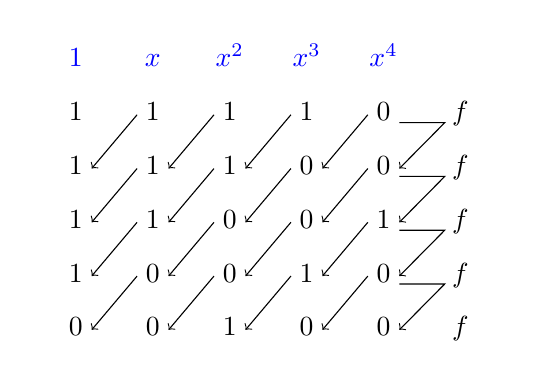
\begin{tikzpicture}
    \matrix [table] (p3)
    {
        {\color{blue}1} & {\color{blue}$x$} & {\color{blue}$x^2$} & {\color{blue}$x^3$} & {\color{blue}$x^4$} & \\
        1 & 1 & 1 & 1 & 0 & $f$ \\
        1 & 1 & 1 & 0 & 0 & $f$ \\
        1 & 1 & 0 & 0 & 1 & $f$ \\
        1 & 0 & 0 & 1 & 0 & $f$ \\
        0 & 0 & 1 & 0 & 0 & $f$ \\
    };
    \foreach \i in {2, 3, 4, 5}
    {   
        \pgfmathtruncatemacro{\ii}{\i+1}
        \foreach \x in {2, 3, 4, 5}
        {
            \pgfmathtruncatemacro\xx{\x-1}
            \draw [->] ($(p3-\i-\x.center)+(-.2cm,0)$) -- ($(p3-\ii-\xx.center)+(.2cm,0)$);
        }
        \draw [->] ($(p3-\i-5.center)+(.2cm,-.1cm)$) -- ($(p3-\i-6.center)+(-.2cm,-.1cm)$) -- ($(p3-\ii-5.center)+(.2cm, 0)$);
    }
    
\end{tikzpicture}
\end{document}